\documentclass[11pt]{article}

\usepackage[utf8]{inputenc}
\usepackage[margin=1in]{geometry}
\usepackage{amsmath,amssymb}
\usepackage{booktabs}
\usepackage{graphicx}
\usepackage{caption}
\usepackage{siunitx}
\usepackage[hidelinks]{hyperref}

\graphicspath{{../results/figures/}}

\title{\textbf{volbench}: An Out-of-Sample Benchmark for\\ Realized-Volatility Forecasting}
\author{Batuhan Boztepe}
\date{\today}

\begin{document}
\maketitle

\begin{abstract}
We benchmark nine volatility forecasters out of sample on real 5-minute
realized data for eight international equity indices (Oxford-Man Institute
Realized Library, 2000--2022), under a strict look-ahead-free expanding-window
design and proxy-robust loss functions \cite{patton2011}. Significance is assessed
with the Diebold--Mariano test \cite{dm1995} and the Model Confidence Set \cite{hln2011}. The central finding is that a \emph{log-space HAR} is in the 90\%
Model Confidence Set for all eight indices at horizons of 1, 5 and 22 days and
is the single best model in most index-horizon cells; a gradient-boosted model
is competitive but does not displace it. Within the HAR family, log
specifications dominate level ones, and a semivariance HAR (LogSHAR) and a
continuous/jump HAR (LogHAR-CJ) edge plain log-HAR. Adding peer indices' lagged
realized variance significantly improves every index's forecast. An
economic-value layer shows that statistical wins do not mechanically become
economic wins. We extend the benchmark, under an internal pre-specified protocol,
into a cross-asset study spanning crypto, futures and FX: log-HAR's dominance
replicates broadly, the only genuine break being gold at the monthly horizon,
alongside a siloed value-at-risk layer in which a leverage-aware GJR-GARCH is the
best engine yet the dynamic-quantile test stays unsolved. All realized estimators
are validated against simulated ground truth, and everything is reproducible
offline from a fixed seed.
\end{abstract}

\section{Introduction}
Volatility forecasting is usually demonstrated by fitting a model and eyeballing
the fit. The deployment-relevant question is different: \emph{which} models win
out of sample, and are the differences statistically meaningful or just noise?
We answer this with (i) microstructure-grade realized estimators validated on
simulation \cite{abdl2003,ab1998}, (ii) a direct multi-horizon walk-forward that rules out look-ahead
bias, (iii) loss functions that rank forecasts consistently despite a noisy
variance proxy, and (iv) formal model-comparison tests. The benchmark is fully
reproducible and ships with the data.

\section{Data}
We use a bundled subset of the Oxford-Man Institute Realized Library \cite{omi2009}: daily
realized measures for eight indices (\texttt{.SPX}, \texttt{.DJI},
\texttt{.FTSE}, \texttt{.GDAXI}, \texttt{.FCHI}, \texttt{.STOXX50E},
\texttt{.N225}, \texttt{.HSI}) from 2000-01-03 to 2022-02-25 (about 5{,}400--5{,}650
trading days each). The file carries 5-minute realized variance (\texttt{rv5}),
its subsampled version, bipower variation, median realized variance, the Parzen
realized kernel \cite{bnhls2008}, downside realized semivariance \cite{ps2015}, and close prices. All measures
are \emph{variances} (decimal returns\textsuperscript{2}, daily); the loader
checks that the implied annualised volatility lands in a plausible band rather
than re-scaling. The library has no realized-quarticity column and no raw
intraday returns, so HARQ \cite{bpq2016} and the jump test \cite{abd2007} are exercised on simulation only.

\section{Methodology}
\paragraph{Target.} Every model forecasts the same quantity: the average
daily variance over the next $h$ days, $\text{target}_t = \frac{1}{h}\sum_{i=1}^{h}\text{RV}_{t+i}$.
Losses are then directly comparable.
\paragraph{No look-ahead.} At origin $t$, a regression model trains only on rows
$s$ whose realization window has closed, i.e. $s + h \le t$. This is enforced in
code and unit-tested for every model (a common silent bug when $h>1$).
\paragraph{Positivity.} Variance forecasts must be strictly positive. Models
that are additive and unbounded (trees, level regressions at long horizons) are
fit in log-variance space and mapped back with the lognormal correction
$\exp(\hat\mu + \tfrac12 \hat\sigma^2)$.
\paragraph{Robust losses.} We rank only with QLIKE,
$L = \sigma^2/h - \log(\sigma^2/h) - 1$, and squared error on the variance
scale; both are consistent under a noisy proxy \cite{patton2011}. RMSE on the
volatility scale is reported for reference but never used to rank.
\paragraph{Significance.} Pairwise equality of predictive accuracy is tested
with the Diebold--Mariano test \cite{dm1995} using a Newey--West HAC variance and the
Harvey--Leybourne--Newbold small-sample correction \cite{hln1997}. The Model Confidence Set
(MCS) \cite{hln2011} uses the range statistic with a moving-block bootstrap (2{,}000
replications); we report the 90\% set.

\section{Estimator validation}
Because the data ships measures rather than intraday returns, the estimators are
validated on 4{,}000 simulated days from an exponential-OU stochastic-volatility
model with optional jumps and microstructure noise, where the integrated and
jump variation are known. Table~\ref{tab:val} shows each estimator recovers its
target. Figure~\ref{fig:sig} is the volatility signature plot: under additive
noise realized variance explodes at high frequency while the realized kernel
stays on the true quadratic variation.

\begin{table}[h]
\centering
\caption{Estimator validation against simulated ground truth (4{,}000 days).}
\label{tab:val}
\begin{tabular}{lrr}
\toprule
Check & Result & Target \\
\midrule
Realized variance / quadratic variation & 1.000 & 1.0 \\
Bipower variation / integrated variance (clean) & 0.998 & 1.0 \\
Median RV / integrated variance & 0.998 & 1.0 \\
Bipower variation / integrated variance (with jumps) & 1.044 & n/a (finite-$M$ bias) \\
(RV $-$ bipower) / jump variation & 0.926 & $\approx$1.0 \\
Realized kernel / QV (clean) & 1.003 & 1.0 \\
Realized variance / QV (with noise) & 3.00 (inflated) & n/a \\
Realized kernel / QV (with noise) & 1.008 (robust) & 1.0 \\
Jump-test false-positive rate @ 5\% & 0.052 & 0.05 \\
Jump-test detection rate (injected) & 0.938 & high \\
\bottomrule
\end{tabular}
\end{table}

\begin{figure}[h]
\centering
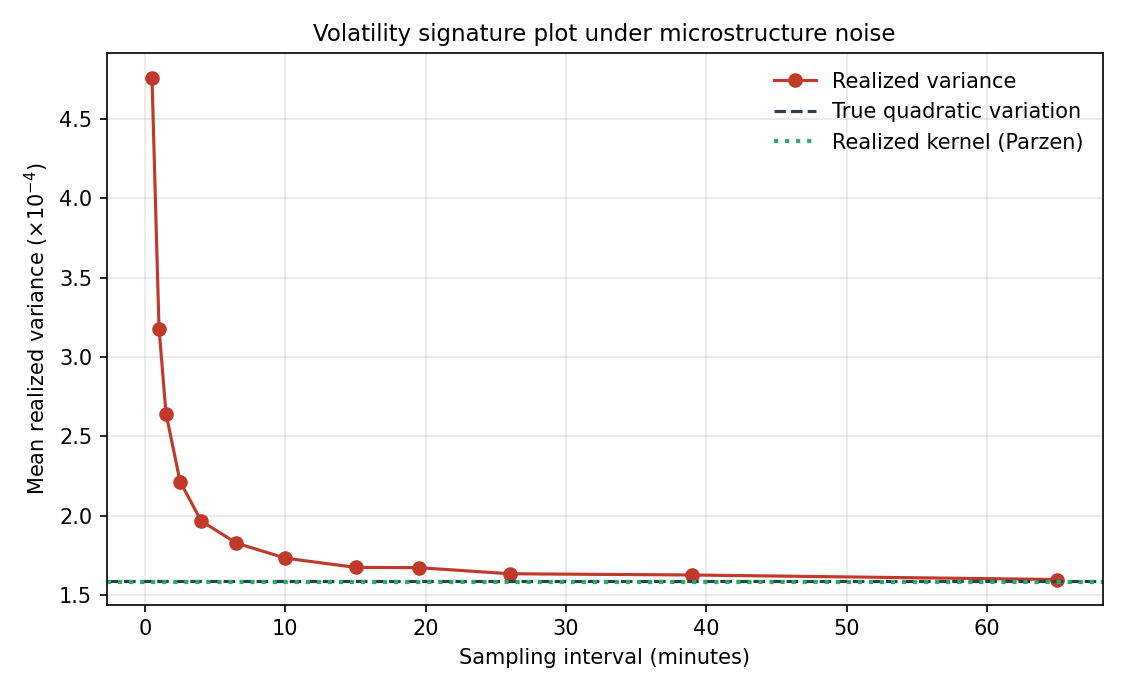
\includegraphics[width=0.8\textwidth]{signature_plot.png}
\caption{Volatility signature plot under microstructure noise. Realized
variance is biased upward at high frequency; the realized kernel tracks the true
quadratic variation across sampling intervals.}
\label{fig:sig}
\end{figure}

\section{Main benchmark (Track 1)}
Table~\ref{tab:main} reports out-of-sample QLIKE for the full suite at the
one-day horizon, averaged over the eight indices, with the average rank, the
number of indices in the 90\% MCS, and the number where the model significantly
beats level-HAR. Log-HAR \cite{corsi2009} leads at every horizon and is in the MCS for all eight
indices at $h \in \{1,5,22\}$; the gradient-boosted model and the long-memory
ARFIMA are the closest non-HAR competitors (GBRT runner-up at $h=5$, ARFIMA at
$h=22$), but neither displaces log-HAR. Figure~\ref{fig:lead} and Figure~\ref{fig:hz} visualise the ranking
and its stability across horizons.

\begin{table}[h]
\centering
\caption{Track 1 leaderboard, $h=1$ (8 indices, $\approx$5{,}000 origins each).}
\label{tab:main}
\begin{tabular}{lrrrr}
\toprule
Model & Avg QLIKE & Avg rank & MCS (of 8) & Beats HAR \\
\midrule
\textbf{log-HAR} & \textbf{0.187} & \textbf{1.12} & \textbf{8} & 6 \\
GBRT (log) & 0.196 & 2.75 & 1 & 2 \\
ARFIMA (log) & 0.197 & 2.75 & 0 & 4 \\
HAR & 0.198 & 3.38 & 2 & n/a \\
AR(1)-log & 0.239 & 5.50 & 0 & 0 \\
EWMA & 0.244 & 5.88 & 0 & 0 \\
MA(22) & 0.262 & 7.00 & 0 & 0 \\
Random walk & 0.468 & 7.75 & 0 & 0 \\
Historical mean & 0.651 & 8.88 & 0 & 0 \\
\bottomrule
\end{tabular}
\end{table}

At $h=5$, log-HAR is significantly better than level-HAR on all eight indices
(avg QLIKE 0.140 vs 0.160). At $h=22$ it remains rank-1 and in the MCS for all
eight (avg QLIKE 0.197). The naive baselines (random walk, historical mean,
moving average, EWMA) are dominated throughout.

\begin{figure}[h]
\centering
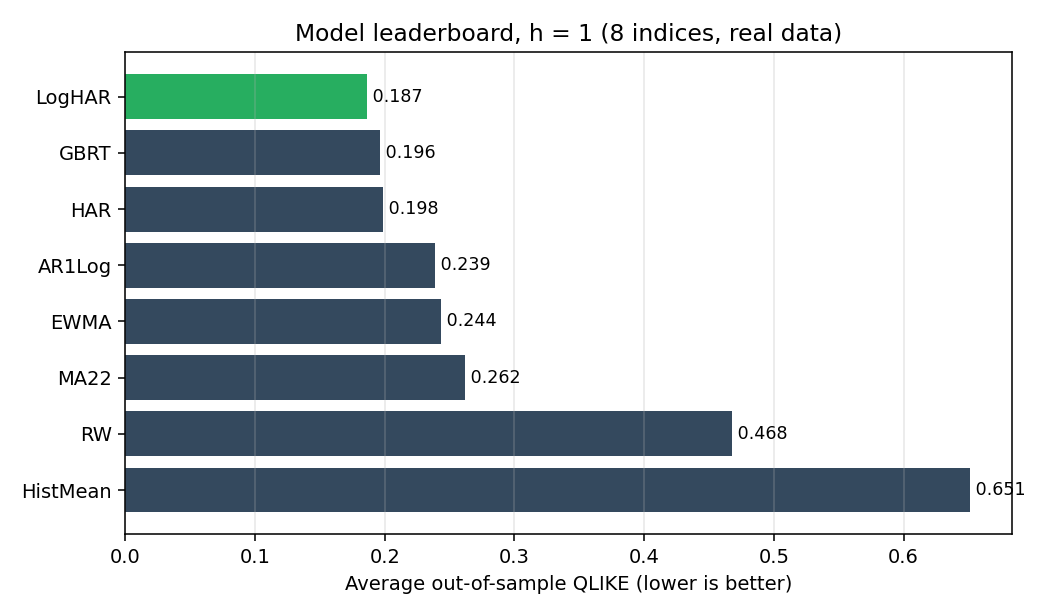
\includegraphics[width=0.74\textwidth]{leaderboard_h1.png}
\caption{Average out-of-sample QLIKE by model at $h=1$.}
\label{fig:lead}
\end{figure}

\begin{figure}[h]
\centering
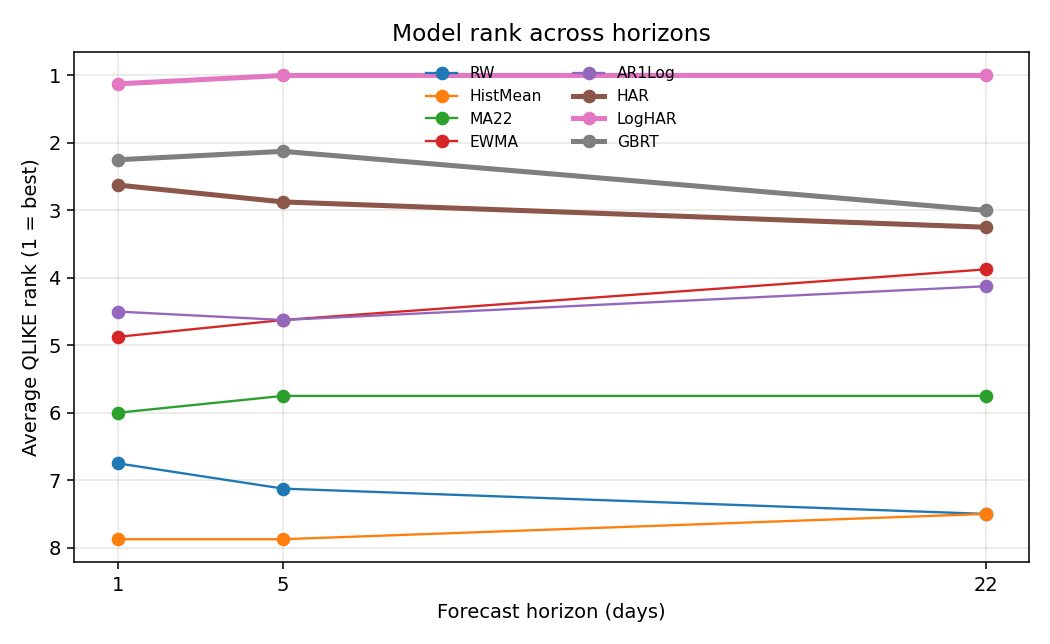
\includegraphics[width=0.74\textwidth]{qlike_by_horizon.png}
\caption{Average QLIKE rank by model across horizons (1 = best). The HAR family
is stable on top at every horizon.}
\label{fig:hz}
\end{figure}

\section{Which HAR variant wins?}
Using real bipower variation \cite{bns2004}, jump variation and realized semivariances, we
compare HAR-J, HAR-CJ (continuous/jump split) \cite{abd2007} and SHAR (semivariance HAR)
\cite{ps2015}, each in level and log form, benchmarked against log-HAR \cite{corsi2009}
(Table~\ref{tab:har}).
Two robust conclusions emerge: log specifications dominate the corresponding
level specifications, and the semivariance HAR (LogSHAR) and continuous/jump HAR
(LogHAR-CJ) edge plain log-HAR. The downside-semivariance ``leverage'' channel
carries genuine predictive content. Level measure-HAR models can produce
non-positive or wildly extrapolated forecasts, which is precisely why the log
forms are preferred.

\begin{table}[h]
\centering
\caption{HAR-family average QLIKE rank (8 indices); lower is better. MCS is the
count of indices in the 90\% set.}
\label{tab:har}
\begin{tabular}{lrrrrrr}
\toprule
 & \multicolumn{2}{c}{$h=1$} & \multicolumn{2}{c}{$h=5$} & \multicolumn{2}{c}{$h=22$} \\
Model & rank & MCS & rank & MCS & rank & MCS \\
\midrule
LogSHAR    & 2.50 & 7 & 1.50 & 7 & 1.50 & 8 \\
LogHAR-CJ  & 2.25 & 5 & 1.75 & 7 & 2.50 & 7 \\
LogHAR     & 3.50 & 2 & 3.12 & 1 & 2.50 & 4 \\
LogHAR-J   & 4.25 & 2 & 3.62 & 2 & 3.50 & 4 \\
SHAR       & 6.12 & 1 & 5.62 & 0 & 5.62 & 2 \\
HAR-J      & 4.50 & 2 & 6.00 & 1 & 6.12 & 1 \\
HAR        & 6.62 & 1 & 7.38 & 0 & 7.00 & 1 \\
HAR-CJ     & 6.25 & 1 & 7.00 & 1 & 7.25 & 0 \\
\bottomrule
\end{tabular}
\end{table}

\section{Does machine learning win on richer features?}
The headline uses a single gradient-boosted model on plain HAR features. We
sharpen the "ML vs HAR" question with LightGBM and XGBoost (the appropriate
learners for tabular HAR features at this data size; a feed-forward MLP was also
tested but is data-starved and unstable on $\approx$5{,}000 daily observations),
each fit in log-variance space with hyperparameters chosen by a \emph{strict
expanding-window inner cross-validation} that only sees data available at the
origin. That removes leakage, the single most common silent error in ML volatility
studies. We test both a plain HAR feature set and an enriched set that adds the
continuous/jump decomposition and the realized semivariances.

The conclusions are robust. At the weekly and monthly horizons log-HAR
is rank-1 and in the Model Confidence Set for all eight indices, while no ML model
enters the MCS for any index. At the daily horizon a log-HAR\,+\,LightGBM
combination edges log-HAR on average but beats it significantly on only one of
eight indices (Diebold--Mariano, 5\%), so the two are statistically
indistinguishable \cite{dm1995}. Crucially, enriching the ML feature set with realized measures
does \emph{not} help: the plain-to-enriched change is a marginal $+1.9\%$ at
$h=1$ but $-3.3\%$ and $-6.8\%$ at $h=5$ and $h=22$. The extra features
\emph{hurt} the learner at longer horizons (overfitting). On \texttt{.SPX} at
$h=1$, log-HAR scores QLIKE 0.206 against 0.233 (LightGBM, enriched) and 0.219
(XGBoost, enriched). With leakage controlled and features made rich, structure
still beats flexibility on daily realized variance; cross-asset enrichment is
examined separately below.

\begin{table}[h]
\centering
\caption{ML vs log-HAR: average QLIKE rank (8 indices) and MCS count. ``Combo''
is the equal-weight log-HAR\,+\,LightGBM-enriched forecast.}
\label{tab:ml}
\begin{tabular}{lrrrrrr}
\toprule
 & \multicolumn{2}{c}{$h=1$} & \multicolumn{2}{c}{$h=5$} & \multicolumn{2}{c}{$h=22$} \\
Model & rank & MCS & rank & MCS & rank & MCS \\
\midrule
log-HAR        & 1.62 & 7 & 1.25 & 8 & 1.12 & 8 \\
Combo          & 1.38 & 7 & 1.75 & 6 & 1.88 & 4 \\
XGBoost (enr.) & 3.00 & 3 & 3.25 & 0 & 3.62 & 0 \\
LightGBM (plain)& 4.75 & 0 & 3.88 & 0 & 3.62 & 0 \\
LightGBM (enr.)& 4.25 & 0 & 4.88 & 0 & 4.75 & 0 \\
\bottomrule
\end{tabular}
\end{table}

\section{Cross-index spillover}
Does a target index benefit from its peers? We augment a log-HAR for each target
with the other seven indices' lagged daily realized variance (CrossHAR) and test
it against own-information log-HAR. CrossHAR lowers QLIKE for all eight indices,
by roughly 1.7--8\% at $h=1$ (largest for \texttt{.FTSE}, $\approx$8\%, and
\texttt{.STOXX50E}). Because CrossHAR \emph{nests} log-HAR, the standard
Diebold--Mariano test is not valid for this comparison \cite{diebold2015}; we
therefore judge significance with the Clark--West \cite{clarkwest2007} nested-model test on the
MSE channel. By that test CrossHAR significantly improves on log-HAR for seven of
the eight indices at $h=1$ (all except \texttt{.SPX}) and four of eight at
$h=5$. Volatility spillover across major
equity markets is real and largely exploitable out of sample, strongest at the
daily horizon.

\section{Economic value}
Statistical accuracy is translated into money and risk three ways: a
volatility-targeting strategy (scale exposure by $\text{target vol}/\text{forecast vol}$),
normal-VaR exceedance backtests \cite{kupiec1995,christoffersen1998}, and a
Black--Scholes option-pricing loss. The statistically-best model is \emph{not} a
clean economic winner: log-HAR delivers the most accurate option prices, but a
simple EWMA edges it on vol-targeted Sharpe, and \emph{all} models under-cover
5\% VaR (empirical exceedances $\approx$6--13\%) because a Gaussian quantile
ignores the fat tails of daily index returns. A QLIKE leaderboard alone would hide this.

\section{Regime analysis}
Because the data is dated, we split 2000--2022 into calm vs turbulent states
(median realized-variance cut, conditioned only on information known at the
origin) and into the GFC and COVID crisis windows, then re-run the MCS within
each subsample. Log-HAR stays rank-1 and in the MCS for all eight indices in the
calm, turbulent and GFC regimes. The COVID window is the exception: with only
$\approx$93 origins per index the MCS cannot separate the models (all are
retained for all eight indices) and level-HAR nominally edges log-HAR,
a sample-size effect, not evidence against log-HAR. The most striking pattern is
that the gap to the naive baselines \emph{widens} sharply in crises: the
historical mean's QLIKE is about $3.5\times$ log-HAR's over the full sample but
$\approx 12\times$ during the GFC and $\approx 7\times$ during COVID. Getting the
persistence of variance right matters most exactly when risk is highest.

\section{Track 2: GARCH on returns (kept separate)}
For reference we run GARCH(1,1) \cite{bollerslev1986}, GJR-GARCH \cite{gjr1993}, RiskMetrics and a constant-variance
benchmark on real S\&P 500 daily returns, scoring one-step variance forecasts
against the squared daily return. GJR-GARCH wins (QLIKE 1.72, the sole MCS
member), ahead of GARCH (1.75), RiskMetrics (1.80) and constant variance (2.36).
These QLIKE \emph{levels} are an order of magnitude above Track 1's ($\approx$0.2)
purely because the squared-return proxy is far noisier than 5-minute realized
variance. That is exactly why the two tracks must never be compared directly.

\section{From forecast to edge}
A good realized-variance forecast is not alpha by itself; it monetises through a
tradable volatility instrument and through risk control. Three results connect
the benchmark to deployment.

\paragraph{Fat-tailed VaR.} Daily index returns are heavy-tailed, so a Gaussian
value-at-risk under-covers: on real index data the normal $5\%$ VaR is breached on
about $9.1\%$ of days (log-HAR forecasts, averaged over the eight indices). A
Student-t tail does \emph{not} help, since at the $5\%$ level the unit-variance $t$
quantile is less extreme than the normal, giving $\approx 9.1\%$ exceedances. A
filtered-historical-simulation (FHS) quantile, calibrated out-of-sample on a
leading warm-up block, substantially improves unconditional coverage
($\approx 6.5\%$), but none of the three fully passes the Engle--Manganelli
dynamic-quantile test \cite{engleman2004} on real data: the residual mis-specification lies in the
conditional dynamics (volatility clustering the point forecast misses), not in the
tail shape alone. (On i.i.d.\ heavy-tailed simulation, where the conditional mean
of variance is constant, FHS does recover a $\approx 5\%$ rate.)

\paragraph{The variance risk premium.} The cleanest monetisation of a validated
$E[\text{RV}]$ is the variance risk premium, implied minus realized variance. On
the S\&P 500, average implied volatility (VIX) is $21.5\%$ against $16.3\%$
realized, and the premium is positive on $92\%$ of days. A naive short-variance
book earns an annualised Sharpe of $1.45$; \emph{timing} it with the log-HAR
forecast (scaling the short down when the forecast says implied is only fairly
priced) raises the Sharpe to $1.60$ and cuts maximum drawdown by about
$65\%$. These Sharpes are gross of transaction costs and computed on overlapping
$22$-day variance-swap payoffs, so the absolute levels are inflated relative to a
non-overlapping annualisation \cite{baileylopezdeprado2014}; the meaningful results are the \emph{lift} over the
naive book and the drawdown reduction, both of which survive realistic
variance-swap costs. The naive book earns more absolute dollars (the timed book
deliberately takes less risk), but on a risk-adjusted basis the forecast adds
value.

\paragraph{Volatility targeting.} Scaling exposure by
$\text{target vol}/\text{forecast vol}$, net of transaction costs, holds realised
volatility near target and reduces maximum drawdown by $20$--$49\%$ (median
$\approx 34\%$) versus buy-and-hold ($-0.40$ vs $-0.62$ averaged over the eight
indices, close to halving only on the US indices). It improves
the Sharpe ratio on the US indices, and a jump/regime de-risking overlay trims
drawdown further. On the cross-section a smoother EWMA forecast can
match log-HAR as the sizing input because it turns over less; vol targeting is a
risk-management tool, not free return. The full accounting (costs, turnover,
drawdown, and out-of-sample significance) is the point.

\section{Generality: crypto (Track 3)}
Does the headline survive a completely different asset class? We extend the
benchmark to four crypto assets (BTC, ETH, BNB, SOL) using realized measures
computed from real Binance 5-minute bars. Crypto trades 24/7 and is far more
volatile (annualised realized volatility of $69\%$ for BTC up to $134\%$ for
SOL) with heavier tails. Because the bars are real and high-frequency, this is
also the first track where realized quarticity, and therefore HARQ, runs on
real data, and where the volatility signature plot
(Figure~\ref{fig:cryptosig}) is drawn from genuine microstructure noise rather
than simulation.

The central result generalises: \textbf{log-HAR is rank-1 and in the Model
Confidence Set for all four coins at every horizon} ($h \in \{1,5,22\}$), with
the gradient-boosted model again the runner-up and the naive baselines
dominated. Two contrasts with equities emerge. First, \emph{HARQ does not
transfer}: now that it can be evaluated on real realized quarticity, it is the
worst model on crypto (its daily-coefficient correction is destabilised by the
heavy-tailed crypto quarticity). Second, \emph{cross-coin spillover is weak}:
CrossHAR beats log-HAR only marginally on BTC (Diebold--Mariano $p \approx 0.09$)
and insignificantly on the others, unlike the strong, uniform spillover among
equity indices. The structure that wins is the same (log-space HAR), but the
cross-asset and measurement-error refinements that help (or are neutral) for
equities do not carry over.

One limitation of the crypto panel is \emph{survivorship}: the four coins
(BTC, ETH, BNB, SOL) are large assets selected because they are liquid and still
trading today, so a coin that died (e.g.\ LUNA/Terra) is absent. The result is
therefore that log-HAR generalises to \emph{surviving major} coins, not a claim
over the full, delisting-inclusive cross-section. The equity panel does not share
this issue. It is a fixed set of major indices, which are not delisted for poor
performance.

\begin{figure}[h]
\centering
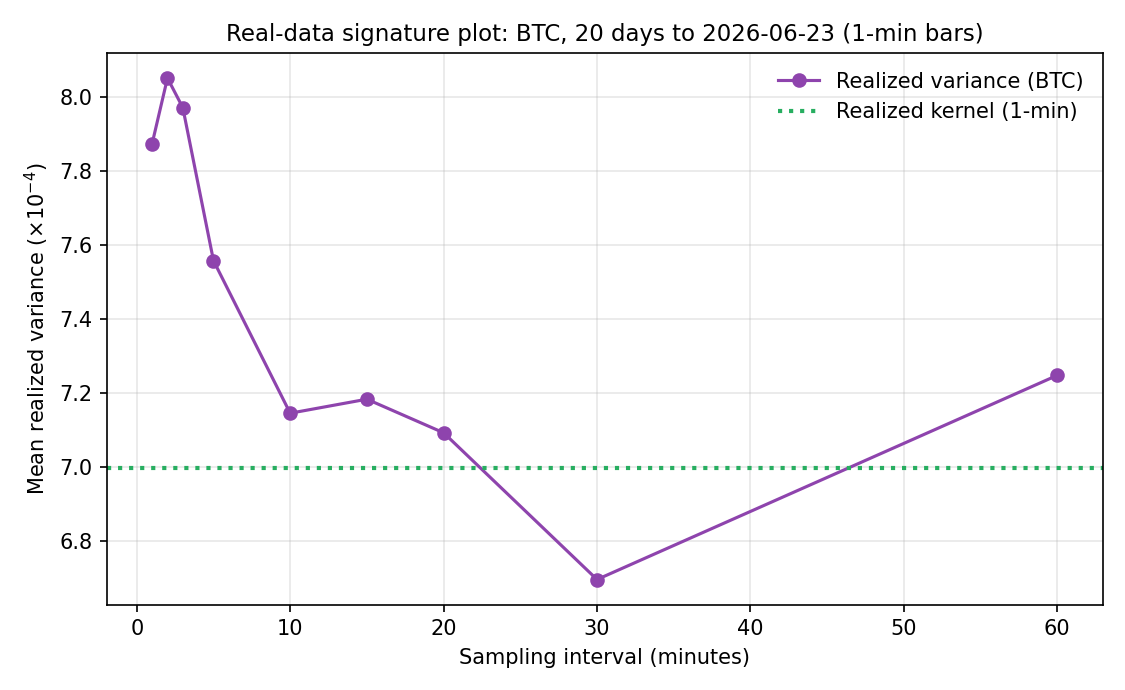
\includegraphics[width=0.78\textwidth]{crypto_signature.png}
\caption{Real-data volatility signature plot: mean BTC realized variance against
sampling interval (1-minute bars). Realized variance is inflated at the highest
frequencies by genuine microstructure noise and settles toward the realized
kernel as the interval coarsens, the same effect demonstrated on simulation in
Figure~\ref{fig:sig}, here on real data.}
\label{fig:cryptosig}
\end{figure}

\section{Cross-asset generalisation (pre-specified protocol)}
The crypto track asks whether the headline survives one new asset class. We then
ask the sharper, falsifiable question: \emph{where does the HAR family stop
winning?} We answer it under an internal, pre-specified protocol: decision rules fixed in advance
as a discipline, author-attested and \emph{not} externally registered or timestamped,
so the answer cannot be reframed after the fact. The pre-specified hypothesis predicts the HAR family
\emph{dominates} mature, calendar-synchronised markets and \emph{degrades} under
reversed leverage, 24/7 calendars, microstructure noise, or event-driven breaks.
The primary deliverable is the Q5 transfer matrix (Figure~\ref{fig:transfer}): the
Liu--Patton--Sheppard ``does anything beat 5-minute RV?'' question applied to
\emph{models}, namely where a HAR-family model stays in the 90\% Model Confidence Set,
by asset class and horizon, across equities, surviving and survivorship-corrected
crypto (4 and 22 coins), VOLARE futures (13: rates, commodity, equity-index, fx)
and VOLARE FX (13: 7 majors, 6 EM/secondary).

The honest result is \textbf{robust replication with narrow cracks}, not a clean
discovery. A HAR-family model is in the MCS and single-best in 8/8 equities, 4/4
and 18--19/22 crypto, both Treasury futures, 37/39 futures cells and 38/39 FX
cells. These counts are robust to the MCS confidence level: re-running the
confirmatory arms at the stricter $\alpha=0.25$ leaves the dominance counts and
every per-instrument verdict unchanged (37/39 and 38/39 at both levels). The
\emph{primary} pre-specified prediction, that rates futures (FV/TY)
would break HAR (with FOMC and auction jumps as the hypothesized driver), was \textbf{falsified}: HAR
dominates both at every horizon (logged as such in the amendment record). The only
genuine degrade is gold (GC) at $h=22$, where the MCS collapses to a single EWMA
(beating the best HAR variant by $\approx 25\%$); it is adversarially robust (seven
seeds, $B \in \{2\text{k}\dots20\text{k}\}$) but isolated, at a secondary horizon,
and partly mechanical (the long-horizon estimation-risk immunity of a
parameter-light smoother), so it does not satisfy the predicted-mechanism clause.
Equity-tuned refinements do not transfer to log-HAR: HARQ never beats log-HAR
outside equities (0/22 crypto, 0/13 futures, 0/13 FX); it does beat plain
(un-logged) HAR in a minority of cells (2/13 futures and 2/13 FX at $h=1$, 5/22
crypto), so the quarticity correction carries some value off-equity but the log
transform already captures it. The LogSHAR semivariance edge vanishes in crypto
(0/22 at $h=1$) while only partly carrying to FX. The
confirmatory outcome is therefore mixed/partial, leaning ``replication at scale'',
a failure mode named in advance, so the contribution is breadth, rigour and
honest negatives rather than a new model or a headline break.

\begin{figure}[h]
\centering
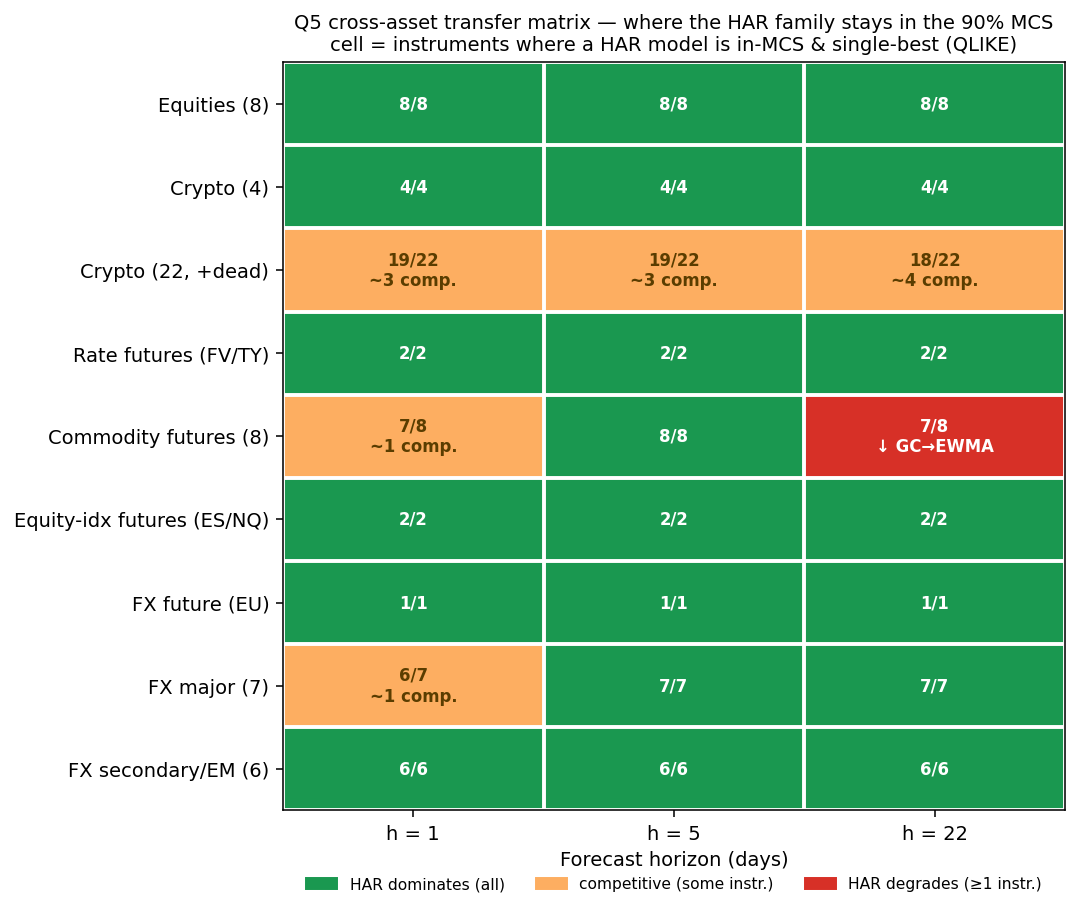
\includegraphics[width=0.86\textwidth]{transfer_matrix.png}
\caption{Q5 cross-asset transfer matrix. Each cell is coloured by its worst
per-instrument state: green if a HAR-family model is in the 90\% MCS and
single-best for every instrument, amber if some are only competitive, red if at
least one shows a genuine degradation. The cell is annotated with the dominate fraction
and the named crack. log-HAR is robust at the level across classes; the single red
cell is gold at the monthly horizon.}
\label{fig:transfer}
\end{figure}

\paragraph{Risk layer: VaR (siloed; an open problem).} A direct-quantile CAViaR
\cite{engleman2004} layer, compared on a common window against same-window
GARCH-family \cite{bollerslev1986,gjr1993} and historical VaR, closes the VaR sub-question directly
(Table~\ref{tab:var}). Normal VaR under-covers the $5\%$ tail ($\approx 9.1\%$
exceedances) and a Student-$t$ tail does not help; filtered historical simulation
improves coverage ($\approx 6.5\%$) but still fails the Engle--Manganelli
dynamic-quantile (DQ) test. CAViaR fixes the coverage but, like FHS, passes DQ on
only one index. The best VaR engine is the leverage-aware GJR-GARCH (DQ pass 3/8,
near-nominal coverage): it is the asymmetry channel, not the modelling paradigm
(direct-quantile versus variance), that matters. Full conditional-quantile
adequacy across twenty years of equity data remains unsolved. This VaR track is
kept strictly separate from the Track-1 QLIKE/MCS ranking.

\begin{table}[h]
\centering
\caption{VaR engines on a common window (8 indices, nominal $5\%$, $h=1$): average
exceedance rate and the number of indices passing the Engle--Manganelli DQ test.
The variance-based GJR-GARCH leads; CAViaR fixes coverage but not the DQ dynamics.}
\label{tab:var}
\begin{tabular}{lrr}
\toprule
VaR engine & Avg exceedance & DQ pass (of 8) \\
\midrule
Normal              & 9.06\% & 0 \\
Student-$t$         & 9.14\% & 0 \\
FHS                 & 6.48\% & 1 \\
RiskMetrics EWMA    & 6.06\% & 0 \\
GARCH               & 5.47\% & 0 \\
\textbf{GJR-GARCH}  & \textbf{5.52\%} & \textbf{3} \\
CAViaR-SAV          & 5.93\% & 0 \\
CAViaR-AS           & 5.56\% & 1 \\
CAViaR-Realized     & 6.07\% & 0 \\
\bottomrule
\end{tabular}
\end{table}

\section{Conclusion}
A correctly specified log-space HAR is hard to beat out of sample: it dominates
naive baselines decisively and is not displaced by a gradient-boosted model on
daily data. The best refinements stay inside the HAR family (log semivariance
and continuous/jump forms) and in cross-asset information (spillover), not in
black-box complexity. Economic-value and regime analyses temper the headline:
statistical wins are necessary but not sufficient for risk and trading use. The
whole pipeline (estimators, simulator, models, tests, and report) is
reproducible offline from a fixed seed.

\section*{Declaration of AI tool usage}
This project was built with Claude Code, Anthropic's agentic coding tool.
The author set the research questions, the methodology, and the pre-specified
decision rules, and reviewed and verified all code and results. The use covered
implementation, refactoring, figure generation, and drafting. Every statistical
result is reproducible from the committed code and a fixed seed. The responsibility
for the final content, analysis, and conclusions rests entirely with me.

\begin{thebibliography}{99}
\bibitem{patton2011} A.~Patton (2011). Volatility forecast comparison using imperfect volatility proxies. \emph{Journal of Econometrics}.
\bibitem{corsi2009} F.~Corsi (2009). A simple approximate long-memory model of realized volatility. \emph{Journal of Financial Econometrics}.
\bibitem{hln2011} P.~Hansen, A.~Lunde, J.~Nason (2011). The Model Confidence Set. \emph{Econometrica}.
\bibitem{bns2004} O.~Barndorff-Nielsen, N.~Shephard (2004). Power and bipower variation with stochastic volatility and jumps. \emph{Journal of Financial Econometrics}.
\bibitem{ps2015} A.~Patton, K.~Sheppard (2015). Good volatility, bad volatility. \emph{Review of Economics and Statistics}.
\bibitem{bpq2016} T.~Bollerslev, A.~Patton, R.~Quaedvlieg (2016). Exploiting the errors: a simple approach for improved volatility forecasting. \emph{Journal of Econometrics}.
\bibitem{omi2009} G.~Heber, A.~Lunde, N.~Shephard, K.~Sheppard (2009). Oxford-Man Institute's Realized Library.
\bibitem{clarkwest2007} T.~Clark, K.~West (2007). Approximately normal tests for equal predictive accuracy in nested models. \emph{Journal of Econometrics}.
\bibitem{diebold2015} F.~Diebold (2015). Comparing predictive accuracy, twenty years later: a personal perspective on the use and abuse of Diebold--Mariano tests. \emph{Journal of Business \& Economic Statistics}.
\bibitem{bnhls2008} O.~Barndorff-Nielsen, P.~Hansen, A.~Lunde, N.~Shephard (2008). Designing realized kernels to measure ex post variation of equity prices in the presence of noise. \emph{Econometrica}, 76(6):1481--1536.
\bibitem{dm1995} F.~Diebold, R.~Mariano (1995). Comparing predictive accuracy. \emph{Journal of Business \& Economic Statistics}, 13(3):253--263.
\bibitem{hln1997} A.~Harvey, S.~Leybourne, P.~Newbold (1997). Testing the equality of prediction mean squared errors. \emph{International Journal of Forecasting}, 13(2):281--291.
\bibitem{kupiec1995} P.~Kupiec (1995). Techniques for verifying the accuracy of risk measurement models. \emph{Journal of Derivatives}, 3(2):73--84.
\bibitem{christoffersen1998} P.~Christoffersen (1998). Evaluating interval forecasts. \emph{International Economic Review}, 39(4):841--862.
\bibitem{engleman2004} R.~Engle, S.~Manganelli (2004). CAViaR: conditional autoregressive value at risk by regression quantiles. \emph{Journal of Business \& Economic Statistics}, 22(4):367--381.
\bibitem{abd2007} T.~Andersen, T.~Bollerslev, F.~Diebold (2007). Roughing it up: Including jump components in the measurement, modelling, and forecasting of return volatility. \emph{Review of Economics and Statistics}, 89(4):701--720.
\bibitem{abdl2003} T.~Andersen, T.~Bollerslev, F.~Diebold, P.~Labys (2003). Modeling and forecasting realized volatility. \emph{Econometrica}, 71(2):579--625.
\bibitem{ab1998} T.~Andersen, T.~Bollerslev (1998). Answering the skeptics: yes, standard volatility models do provide accurate forecasts. \emph{International Economic Review}, 39(4):885--905.
\bibitem{bollerslev1986} T.~Bollerslev (1986). Generalized autoregressive conditional heteroskedasticity. \emph{Journal of Econometrics}, 31(3):307--327.
\bibitem{gjr1993} L.~Glosten, R.~Jagannathan, D.~Runkle (1993). On the relation between the expected value and the volatility of the nominal excess return on stocks. \emph{Journal of Finance}, 48(5):1779--1801.
\bibitem{baileylopezdeprado2014} D.~Bailey, M.~Lopez de Prado (2014). The deflated Sharpe ratio: correcting for selection bias, backtest overfitting, and non-normality. \emph{Journal of Portfolio Management}, 40(5):94--107.
\end{thebibliography}

\end{document}
